\documentclass[../piano_di_progetto.tex]{subfiles}

\begin{document}
In questa sezione verranno illustrati i prospetti orari e relativi costi per le varie fasi di lavoro. Il bilancio si suddivide in:
\begin{itemize}
\item \textbf{Positivo}: se sono state necessarie meno ore di quelle preventivate;
\item \textbf{Paritario}: se sono state svolte effettivamente le ore preventivate;
\item \textbf{Negativo}: se sono state necessarie più ore di quelle preventivate;
\end{itemize}

\subsection{Analisi}%
\label{sub:cons_analisi}
Le ore di lavoro svolte in questa fase sono destinate alla scelta del capitolato e allo studio autonomo, quindi queste ore svolte non verranno rendicontate.\\
Poiché l'analisi dei requisiti è un documento molto importante, ha richiesto l'investimento di molte più ore da parte degli analisti.

\begin{table}[!ht]
	\centering
	\begin{tabular}{|l|c|c|c|c|c|c|c|}
	\hline
	\rowcolor{lightgray}
	\textbf{Nome} & \textbf{Re} & \textbf{Am} & \textbf{An} & \textbf{Pg}  & \textbf{Pr}   & \textbf{Ve} & \textbf{Totale}\\
	\hline
	Contro Daniel Eduardo & 0 & 0 & 16(+3) & 0 & 0 & 15 (+1) & 31(+4) \\
	Fichera Jacopo & 0 & 0 & 16(+3) & 0 & 0 & 15 (+1) & 31(+4) \\
	Kostadinov Samuel & 0 & 10 & 5 & 0 & 0 & 12 & 27 \\			
	Masevski Martin & 4 & 10 & 5 & 0 & 0 & 8 & 27 \\
	Pagotto Manuel & 0 & 0 & 15(+2) & 0 & 0 & 16 (+2) & 31(+4) \\			
	Paparazzo Giorgia & 13 & 0 & 4 & 0 & 0 & 10 & 27 \\
	Rizzo Stefano & 0 & 0 & 16(+4) & 0 & 0 & 15 & 31(+4) \\
	\hline
	\end{tabular}
	\caption{Resoconto orario della fase di Analisi}
\end{table}

\begin{center}
	\begin{longtable}{|l|c|c|}
		\hline
		\rowcolor{lightgray}
		\textbf{Ruolo} & \textbf{Ore} & \textbf{Costo in €}\\
		\hline
		\endhead
		
		\hline
		\multicolumn{3}{|c|}{\emph{Continua alla pagina successiva...}}\\
		\hline
		\endfoot

		\endlastfoot
		Responsabile & 17 & 510,00 \\
		Amministratore & 20 & 400,00 \\
		Analista & 77(+12) & 1.925,00(+300,00 €) \\
		Progettista &    0       & 0 \\
		Programmatore &  0       & 0 \\
		Verificatore &   91(+4)      & 1.365,00 (+60,00€) \\
		\hline
		\textbf{Totale preventivo} & \textbf{189} & \textbf{3.840,00 €} \\
		\hline
		\textbf{Totale consuntivo} & \textbf{205	} & \textbf{4.200,00 €} \\
		\hline
		\textbf{Differenza} & \textbf{+16} & \textbf{+360 €}\\
		\hline
		\rowcolor{white}
		\caption{Resoconto economico nella fase di analisi}
	\end{longtable}
\end{center}

\subsubsection{Conclusioni}%
\label{sub:cons_con_1}
A fronte di una settimana di ritardo nella consegna, si è vista la necessità di aumentare le ore di lavoro di alcuni dei componenti del gruppo, di conseguenza anche il bilancio economico ha visto un aumento di costi. Sebbene il surplus sfori il limite del 5\% stabilito nel \textsc{Piano di Qualifica}, questo costo non intaccherà il budget totale rendicontato perché questa fase non è rendicontata.

\subsubsection{Preventivo a finire}
\label{sub:cons_prev_fine_1}
Uno dei motivi che hanno portato al ritardo è stato il verificarsi di rischi sottovalutati, quali ad esempio l'inesperienza del gruppo con gli argomenti e le tecnologie non affrontate durante il corso di laurea (RR01), oppure l'aver impiegato molto tempo ad accordarsi circa il way of working. Assieme all'inesperienza in progetti di tale portata (RP01, RP02) e all'inesperienza circa gli strumenti scelti (RT01, RO04), lo sviluppo del progetto ha subito ritardo. Nonostante questo mix letale, il ritardo maturato non è grave, e il gruppo prevede di recuperare.
Grazie al fatto che questa fase non è rendicontata, il preventivo finale rimane intaccato. \\ \\

\subsection{Consolidamento dei requisiti}%
\label{sub:cons_cons_req}
Le ore di lavoro svolte in questa fase non verranno rendicontate nel preventivo finale in quanto sono considerate ore di investimento per l'approfondimento personale.\\
Nella tabella che segue vengono riportate le ore di lavoro effettive durante il periodo di consolidamento dei requisiti: \\

\begin{table}[H]
	\centering
	\begin{tabular}{|l|c|c|c|c|c|c|c|}
	\hline
	\rowcolor{lightgray}
	\textbf{Nome} & \textbf{Re} & \textbf{Am} & \textbf{An} & \textbf{Pg}  & \textbf{Pr}   & \textbf{Ve} & \textbf{Totale}\\
	\hline
	Contro Daniel Eduardo & 0 & 0 & 2 & 0 & 0 & 3 & 5 \\
	Fichera Jacopo & 0 & 0 & 2 & 0 & 0 & 3 & 5 \\
	Kostadinov Samuel & 0 & 1 & 1 & 0 & 0 & 3 & 5 \\			
	Masevski Martin & 1 & 0 & 1 & 0 & 0 & 3 & 5 \\
	Pagotto Manuel & 0 & 0 & 2 & 0 & 0 & 3 & 5 \\			
	Paparazzo Giorgia & 1 & 0 & 1 & 0 & 0 & 3 & 5 \\
	Rizzo Stefano & 0 & 0 & 2 & 0 & 0 & 3 & 5 \\
	\hline
	\textbf{Ore totali ruolo} & \textbf{2} & \textbf{1} & \textbf{11} & \textbf{0} & \textbf{0} & \textbf{21} & \textbf{35} \\
	\hline
	\end{tabular}
	\caption{Resoconto orario della fase di consolidamento dei requisiti}
\end{table}

\begin{center}
	\begin{longtable}{|l|c|c|}
		\hline
		\rowcolor{lightgray}
		\textbf{Ruolo} & \textbf{Ore} & \textbf{Costo in €}\\
		\hline
		\endhead
		
		\hline
		\multicolumn{3}{|c|}{\emph{Continua alla pagina successiva...}}\\
		\hline
		\endfoot

		\endlastfoot
		Responsabile & 	 2 	 & 60,00 \\
		Amministratore & 1 	 & 20,00 \\
		Analista & 		11 	 & 275,00 \\
		Progettista &    0   & 0 \\
		Programmatore &  0   & 0 \\
		Verificatore &   21  & 315,00 \\
		\hline
		\textbf{Totale preventivo} & \textbf{35} & \textbf{€ 670,00} \\
		\hline
		\textbf{Totale consuntivo} & \textbf{35} & \textbf{€ 670,00} \\
		\hline
		\textbf{Differenza} & \textbf{0} & \textbf{€ 0}\\
		\hline
		\rowcolor{white}
		\caption{Resoconto economico della fase di consolidamento dei requisiti}
	\end{longtable}
\end{center}

\subsubsection{Conclusioni}%
\label{sub:cons_con_2}
Ogni ruolo coinvolto in questa fase ha rispettato i tempi, rientrando nelle ore preventivate.

\subsubsection{Preventivo a finire}
\label{sub:cons_prev_fine_2}
Rispettando i tempi preventivati non è necessario apportare modifiche al preventivo. \\ \\

\clearpage
\subsection{Progettazione e codifica della technology baseline}%
\label{sub:cons_prog_tech}
Di seguito vengono riportate le ore di lavoro effettivi durante la fase di progettazione e codifica della technology baseline: \\

\begin{table}[!ht]
	\centering
	\begin{tabular}{|l|c|c|c|c|c|c|c|}
	\hline
	\rowcolor{lightgray}
	\textbf{Nome} & \textbf{Re} & \textbf{Am} & \textbf{An} & \textbf{Pg}  & \textbf{Pr}   & \textbf{Ve} & \textbf{Totale}\\
	\hline
	Contro Daniel Eduardo & 0 & 6(-1) & 0 & 8 & 7(+1) & 9 & 30 \\
	Fichera Jacopo & 0 & 0 & 0 & 9(-1) & 9(+2) & 12(-1) & 30 \\
	Kostadinov Samuel & 0 & 0 & 9(+1) & 10(+2) & 0 & 11(-3) & 30 \\			
	Masevski Martin & 8(-3) & 0 & 0 & 0 & 13(+8) & 9(-5) & 30 \\
	Pagotto Manuel & 8(-2) & 0 & 10(+1) & 0 & 0 & 12(+1) & 30 \\			
	Paparazzo Giorgia & 0 & 0 & 7(-3) & 8(+4) & 7(+1) & 8(-2) & 30 \\
	Rizzo Stefano & 0 & 9 & 0 & 6(+2) & 5(+1) & 10(-3) & 30 \\
	\hline
	\textbf{Ore totali ruolo} & \textbf{16(-5)} & \textbf{15(-1)} & \textbf{26(-1)} & \textbf{41(+7)} & \textbf{41(+13)} & \textbf{71(-13)} & \textbf{210} \\
	\hline
	\end{tabular}
	\caption{Resoconto orario della fase di progettazione e codifica della technology baseline}
\end{table}

\begin{center}
	\begin{longtable}{|l|c|c|}
		\hline
		\rowcolor{lightgray}
		\textbf{Ruolo} & \textbf{Ore} & \textbf{Costo in €}\\
		\hline
		\endhead
		
		\hline
		\multicolumn{3}{|c|}{\emph{Continua alla pagina successiva...}}\\
		\hline
		\endfoot

		\endlastfoot
		Responsabile & 	 16(-5) 	 & 480,00(-150,00) \\
		Amministratore & 15(-1) 	 & 300,00(-20,00) \\
		Analista & 		26(-1) 	 & 650,00(-25,00) \\
		Progettista &    41(+7)   & 902,00(+154,00) \\
		Programmatore &  41(+13)   & 615,00(+195,00) \\
		Verificatore &   71(-13)  & 1.065,00(-195,00) \\
		\hline
		\textbf{Totale preventivo} & \textbf{210} & \textbf{€ 4.053,00} \\
		\hline
		\textbf{Totale consuntivo} & \textbf{210} & \textbf{€ 4.012,00} \\
		\hline
		\textbf{Differenza} & \textbf{0} & \textbf{-€ 41,00}\\
		\hline
		\rowcolor{white}
		\caption{Resoconto economico della fase di progettazione e codifica della technology baseline}
	\end{longtable}
\end{center}

\subsubsection{Conclusioni}%
\label{sub:cons_con_3}
In questa fase il gruppo non è riuscito a smaltire il ritardo accumulato nella fase precedente, per questo questo motivo i documenti vengono consegnati con circa una settimana di ritardo rispetto a quello pianificato. \\
Durante questo periodo è stato rispettato il monte ore preventivato. Le ore totali per ogni ruolo hanno subito una sostanziale modifica, di seguito vengono spiegate le motivazioni:
\begin{itemize}
	\item \textbf{Responsabile}: grazie all'ottima collaborazione dei membri del team il responsabile è riuscito a completare il suo lavoro con un risparmio sulle ore preventivate;
	\item \textbf{Amministratore}: l'amministratore ha portato a termine il lavoro in meno tempo rispetto a quello preventivato, riuscendo a risparmiare un'ora di lavoro;
	\item \textbf{Analista}: l'analista è riuscito a portare a termine il proprio lavoro con minor tempo rispetto a quello preventivato, risparmiando un'ora di lavoro;
	\item \textbf{Progettista}: per una più approfondita e dettagliata possibile progettazione del software, il progettista ha richiesto più ore di quelle inizialmente preventivate, influenzando in minima parte il resoconto economico di questo periodo;
	\item \textbf{Programmatore}: per la realizzazione di un prodotto il più possibile stabile e funzionale i programmatori hanno sforato il monte ore preventivato, influenzando in minima parte il resoconto economico di questo periodo. A fronte di ciò sono riusciti a sviluppare un PoC completo che utilizzasse tutte le tecnologie che serviranno per il prodotto finale;
	\item \textbf{Verificatore}: grazie al fatto che i documenti sono stati ben avviati nella precedente fase e alla nuova amministrazione delle repository, il lavoro di verifica si è visto più snello e rapido, risparmiando molte ore.
\end{itemize} 
In conclusione, in questo periodo, sono stati risparmiati € 41,00 rispetto a quello preventivato.

\clearpage
\subsection{Progettazione e codifica di dettaglio}%
\label{sub:cons_prog_dettaglio}

\subsubsection{Variazione pianificazione}
A seguito dell'esito congelato della presentazione della Product Baseline, è stato necessario aumentare il numero di ore per ogni membro del gruppo.\\
Inoltre il gruppo ha deciso di togliere delle ore dal ruolo di \emph{responsabile} per assegnarle ai ruoli del \emph{programmatore} e del \emph{progettista} per i seguenti motivi:
\begin{itemize}
	\item Il gruppo ha necessitato di più ore di quante preventivate per la scrittura del codice, come tracciato nella sezione \S\ref{sub:rischi_rq} Codice \emph{RT01 - Inesperienza del team nell'uso del linguaggio di programmazione}. %TODO Aggiornare questa sezione con i riferimenti all'appendice A - rischi riscontrati
	\item I \emph{progettisti} hanno impiegato più ore di quanto preventivate nella creazione dei diagrammi UML, come tracciato nella sezione \S\ref{sub:rischi_rq} Codice \emph{RT01 - Inesperienza del team nell'uso del linguaggio di programmazione}.
\end{itemize}

\noindent Di seguito vengono riportate le ore di lavoro effettivi durante la fase di progettazione e codifica di dettaglio: \\
\begin{table}[!ht]
	\centering
	\begin{tabular}{|l|c|c|c|c|c|c|c|}
	\hline
	\rowcolor{lightgray}
	\textbf{Nome} & \textbf{Re} & \textbf{Am} & \textbf{An} & \textbf{Pg}  & \textbf{Pr}   & \textbf{Ve} & \textbf{Totale}\\
	\hline
	Contro Daniel Eduardo & 4(-5) & 0 & 0 & 13(+3) & 20(+2) & 13 & 30 \\
	Fichera Jacopo & 0 & 0 & 0 & 17 & 17 & 16 & 30 \\
	Kostadinov Samuel & 4(-6) & 0 & 0 & 10(+2) & 18(+3) & 18(+1) & 30 \\			
	Masevski Martin & 0 & 0 & 5 & 13 & 13 & 19 & 30 \\
	Pagotto Manuel & 3(-5) & 0 & 0 & 11(+2) & 19(+3) & 17 & 30 \\			
	Paparazzo Giorgia & 0 & 6 & 2 & 17 & 10 & 15 & 30 \\
	Rizzo Stefano & 0 & 8 & 0 & 12 & 14 & 16 & 30 \\
	\hline
	\textbf{Ore totali ruolo} & \textbf{11(-16)} & \textbf{14} & \textbf{7} & \textbf{93(+7)} & \textbf{111(+8)} & \textbf{114(+1)} & \textbf{350} \\
	\hline
	\end{tabular}
	\caption{Resoconto orario della fase di progettazione e codifica di dettaglio}
\end{table}

\begin{figure}[H]
	\centering
	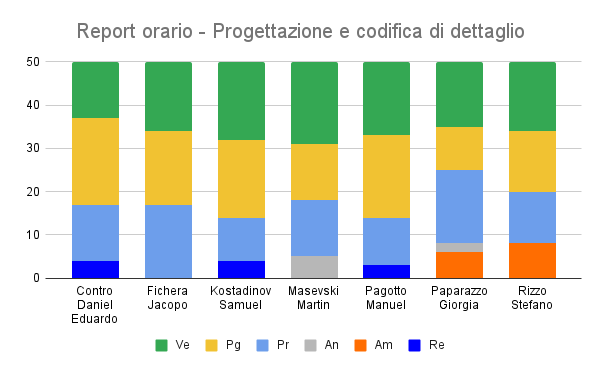
\includegraphics[width=11cm]{src/img/report/report_prog_codifica_dettaglio_consuntivo}
	\caption{Report della suddivisione dei ruoli nella fase di progettazione e codifica di dettaglio}
\end{figure}

\begin{center}
	\begin{longtable}{|l|c|c|}
		\hline
		\rowcolor{lightgray}
		\textbf{Ruolo} & \textbf{Ore} & \textbf{Costo in €}\\
		\hline
		\endhead
		
		\hline
		\multicolumn{3}{|c|}{\emph{Continua alla pagina successiva...}}\\
		\hline
		\endfoot

		\endlastfoot
		Responsabile & 	 11(-16) 	 & 330,00(-480,00) \\
		Amministratore & 14 	 & 280,00 \\
		Analista & 		7 	 & 175,00 \\
		Progettista &    93(+7)   & 2.046,00(+154,00) \\
		Programmatore &  111(+8)   & 1.665,00(+120,00) \\
		Verificatore &   114(+1)  & 1.710,00(+15,00) \\
		\hline
		\textbf{Totale preventivo} & \textbf{350} & \textbf{€ 6.397,00} \\
		\hline
		\textbf{Totale consuntivo} & \textbf{350} & \textbf{€ 6.206,00} \\
		\hline
		\textbf{Differenza} & \textbf{0} & \textbf{-€ 191,00}\\
		\hline
		\rowcolor{white}
		\caption{Resoconto economico della fase di progettazione e codifica di dettaglio}
	\end{longtable}
\end{center}


\subsubsection{Preventivo a finire}
\label{sub:cons_prev_fine_4} 
% In questa fase il bilancio viene chiuso in positivo, sebbene vi sia stato un evidente ritardo nella consegna. Ciò è avvenuto a causa del fatto che il gruppo non è riuscito a rientrare del ritardo maturato inizialmente, inoltre si sono verificati rischi non previsti, ovvero il fatto che la sessione invernale ha richiesto molte risorse da parte di buona parte del gruppo (RO02, RP01). 
% A fronte di ciò, sebbene i documenti siano stati prodotti entro le tempistiche richieste, il PoC ha subito un leggero ritardo, quindi il gruppo ha avuto la necessità di chiedere il colloquio per la Technology Baseline il giorno 8 marzo. Questo ha portato alla possibilità di poter sviluppare più funzionalità di quelle che ci eravamo prefissati, e potenzialmente anticipare parte del lavoro che avverrà nella fase di Progettazione di Dettaglio. 
% Sebbene questa fase sia rendicontata, attualmente il budget finale non ha subito aumenti di prezzo, bensì un leggero risparmio. Il gruppo farà tesoro di questa possibilità e cercherà di trarne vantaggio per la successiva fase.
Avendo risparmiato 41,00 € nella fase precedente, il bilancio del gruppo è in positivo di 232,00 €. Questo è dovuto alla ridistribuzione delle ore nella fase di \emph{Progettazione e codifica di dettaglio}. Le ore assegnate ai ruoli ti \emph{amministratore} e \emph{responsabile} sono ritenute eccessive, al contrario invece, sono necessarie più ore assegnate al ruolo di \emph{programmatore}. A fronte di ciò abbiamo deciso di togliere alcune ore ai ruoli dell'\emph{amministratore} e del \emph{responsabile}, aggiungendone a quello del \emph{programmatore}. 

\paragraph{Preventivo a finire - Validazione e collaudo}

\subparagraph{Prospetto orario}
Di seguito la distribuzione orario della fase di Validazione e collaudo:
\begin{center}
	\begin{longtable}{|l|c|c|c|c|c|c|c|}
		\hline
		\rowcolor{lightgray}
		\textbf{Nome} & \textbf{Re} & \textbf{Am} & \textbf{An} & \textbf{Pg}  & \textbf{Pr}   & \textbf{Ve} & \textbf{Totale} \\

		\hline
			Contro Daniel Eduardo & 0 & 0 & 0 & 0 & 7 & 13 & 20\\
			Fichera Jacopo & 4(-5) & 2(-2) & 0 & 0 & 5(+5) & 9(+2) & 20 \\ 
			Kostadinov Samuel & 0 & 0 & 0 & 10 & 2 & 8 & 20 \\ 		
			Masevski Martin & 0 & 0 & 0 & 5 & 0 & 15 & 20 \\
			Pagotto Manuel & 0 & 2(-2) & 0 & 6 & 2(+2) & 10 & 20 \\			
			Paparazzo Giorgia & 0 & 0 & 0 & 4 & 4 & 12 & 20 \\
			Rizzo Stefano & 3(-5) & 0 & 2 & 0 & 5(+5) & 10 & 20 \\
			\hline
			\textbf{Ore totali ruoli} & \textbf{7(-10)} & \textbf{4(-4)} & \textbf{2} & \textbf{25} & \textbf{25(+12)} & \textbf{77(+2)} & \textbf{140} \\
			\hline
		\rowcolor{white}
		\caption{Preventivo a finire progettazione e codifica di dettaglio - Distribuzione oraria validazione e collaudo}
	\end{longtable}
\end{center}

\begin{figure}[H]
	\centering
	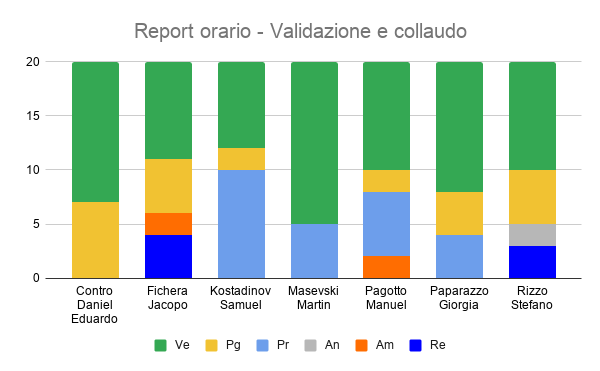
\includegraphics[width=11cm]{src/img/report/report_validazione_collaudo_consuntivo}
	\caption{Preventivo a finire - Report della suddivisione oraria dei ruoli nella fase di validazione e collaudo}
\end{figure}

\subparagraph{Prospetto Economico}

\begin{center}
	\begin{longtable}{|l|c|c|}
		\hline
		\rowcolor{lightgray}
		\textbf{Ruolo} & \textbf{Ore} & \textbf{Costo in €}\\

		\hline
		Responsabile & 7(-10) & 210,00(-300,00)\\
		Amministratore & 4(-4) & 40,00\\
		Analista & 2 & 50,00\\
		Progettista & 25 & 550,00\\
		Programmatore & 25(+12) & 375,00(+180,00)\\
		Verificatore & 77(+2) & 1.155,00(+30,00)\\
		\hline
		\textbf{Totale} & 140 & 2.420,00(-170,00)\\
		\hline
		\rowcolor{white}
		\caption{Preventivo a finire progettazione e codifica di dettaglio - Ore e costo per ruolo validazione e collaudo}
	\end{longtable}
\end{center}


\subsubsection{Conclusioni}%
\label{sub:cons_con_4}
%TODO AGGGIORNARE UNA VOLTA SETTATE LE ORE CONSUNTIVATE PER QUESTA FASE!!!!!!!!!
Il totale delle ore rendicontate preventivate per il progetto diventano le seguenti:
\begin{center}
	\begin{longtable}{|l|c|c|c|c|c|c|c|}
		\hline
		\rowcolor{lightgray}
		\textbf{Nome} & \textbf{Re} & \textbf{Am} & \textbf{An} & \textbf{Pg}  & \textbf{Pr}   & \textbf{Ve} & \textbf{Totale} \\

		\hline
			Contro Daniel Eduardo & 4(-5) & 6(-1) & 0 & 21(+3) & 34(+3) & 35 & 100 \\
			Fichera Jacopo & 4(-5) & 2(-2) & 0 & 26(-1) & 31(+7) & 37(+1) & 100 \\
			Kostadinov Samuel & 4(-6) & 0 & 9(+1) & 30(+4) & 20(+3) & 37(-2) & 100 \\		
			Masevski Martin & 8(-3) & 0 & 5 & 18 & 26(+8) & 43(-5) & 100 \\
			Pagotto Manuel & 11(-7) & 2(-2) & 10(+1) & 17(+2) & 21(+5) & 39(+1) & 100 \\			
			Paparazzo Giorgia & 0 & 6 & 9(-3) & 29(+4) & 21(+1) & 35(-2) & 100 \\
			Rizzo Stefano & 3(-5) & 17 & 2 & 18(+2) & 24(+6) & 36(-3) & 100 \\
			\hline
			\textbf{Ore totali ruolo} & \textbf{34(-31)} & \textbf{33(-5)} & \textbf{35(-1)} & \textbf{159(+14)} & \textbf{177(+33)} & \textbf{262(-10)} & \textbf{700} \\
		\hline	
		\rowcolor{white}
		\caption{Preventivo a finire progettazione e codifica di dettaglio - Distribuzione oraria delle ore totali rendicontate}
	\end{longtable}
\end{center}

\begin{figure}[H]
	\centering
	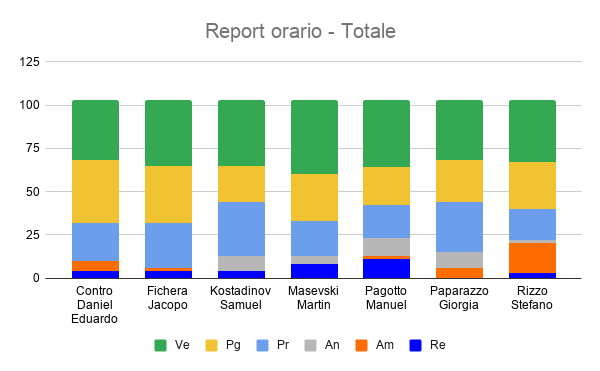
\includegraphics[width=12cm]{src/img/report/Report_totale}
	\caption{Report orario della suddivisione dei ruoli a finire}
\end{figure}


Di seguito il grafico che espone lo scostamento tra le ore preventivate e le ore ore consuntivate:

\begin{figure}[H]
	\centering
	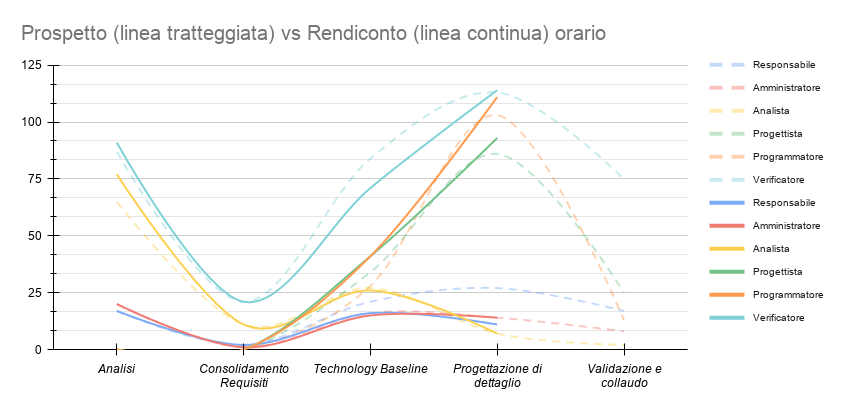
\includegraphics[width=17cm]{src/img/report/prospetto_ore_totale}
	\caption{Scostamento tra ore preventivate a finire e ore consuntivate}
\end{figure}

Di seguito lo spaccato per ruolo di ore e costi:
\begin{center}
	\begin{longtable}{|l|c|c|}
		\hline
		\rowcolor{lightgray}
		\textbf{Ruolo} & \textbf{Ore} & \textbf{Costo in €}\\
		\hline
		
		Responsabile & 34(-31) & 1.020,00(-930,00) \\
		Amministratore & 33(-5) & 660,00(-100,00) \\
		Analista & 35(-1) & 875,00(-25,00) \\
		Progettista & 159(+14) & 3.498,00(+308,00) \\
		Programmatore & 177(+33) & 2.655,00(+495,00) \\
		Verificatore & 262(-10) & 3.930,00(-150,00) \\
		\hline
		\textbf{Totale} & \textbf{700} & \textbf{12.638,00(-402,00)}\\
		\hline
		\rowcolor{white}
		\caption{Preventivo a finire progettazione e codifica di dettaglio - Prospetto dei costi delle ore rendicontate}
	\end{longtable}
\end{center}

Di seguito il grafico che espone lo scostamento tra i costi preventivati e i costi consuntivati:

\begin{figure}[H]
	\centering
	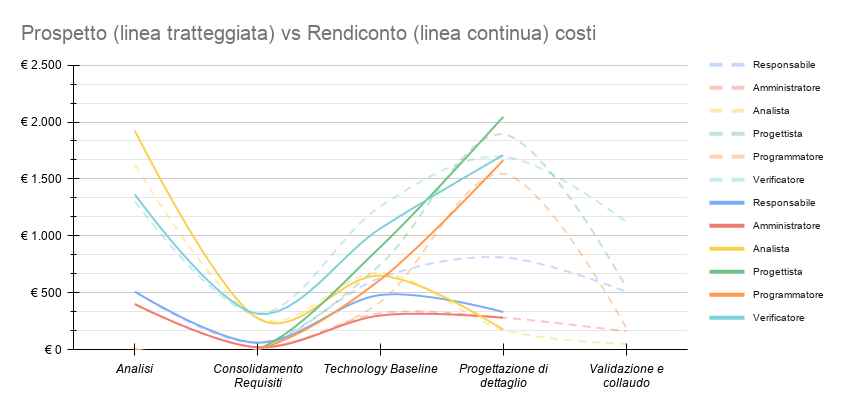
\includegraphics[width=17cm]{src/img/report/prospetto_costi_totale}
	\caption{Scostamento tra costi preventivati a finire e costi consuntivati}
\end{figure}

\noindent Il carico di ore per persona è rimasto invariato, tuttavia togliendo alcune ore ai ruoli di \textsc{amministratore} e \textsc{responsabile} il preventivo è sceso di 402,00 €.\\
Il preventivo a finire è ora di 12.638,00 €. 

\end{document}